\documentclass[aspectratio=169,11pt]{beamer}
\usepackage[T1]{fontenc}
\usepackage[spanish]{babel}
\usepackage[utf8]{inputenc}

\usepackage{pgf,pgfpages}
\usepackage{pgffor} % For loops

\usepackage{tikz}
\usetikzlibrary{arrows,shapes,backgrounds,calc}

\usepackage{graphicx}
\usepackage{wrapfig}
\usepackage{colortbl}
\usepackage{units}

% \usepackage{calrsfs}
% \DeclareMathAlphabet{\pazocal}{OMS}{zplm}{m}{n}
% \usepackage{calligra}
\usepackage[cal=boondox,scaled=1.15]{mathalfa}
% \usepackage{bickham}
% \usepackage{boondox-cal}
% \usepackage{boondox-calo}
% \usepackage{dutchcal}

%% Beamer style >>>>>>>>>>>>>>>>>>>>>>>>>
\mode<presentation>
{
  \usetheme{PHD}
  \setbeamercovered{transparent}
  \setbeamertemplate{items}[square]
}

%\usefonttheme[onlymath]{serif}

\beamertemplatenavigationsymbolsempty

\defbeamertemplate{enumerate item}{mycircle}
{
  %\usebeamerfont*{item projected}%
  \usebeamercolor[bg]{item projected}%
  \begin{pgfpicture}{0ex}{0ex}{1.5ex}{0ex}
    \pgfcircle[fill]{\pgfpoint{-0.1pt}{.65ex}}{1.1ex}
    \pgfbox[center,base]{\color{PHDyellow}{\insertenumlabel}}
  \end{pgfpicture}%
}
[action]
{\setbeamerfont{item projected}{size=\scriptsize}}
\setbeamertemplate{enumerate item}[mycircle]

\setbeamertemplate{frametitle}{\vspace{1.4cm}\structure{\insertframetitle}}
\setbeamertemplate{frametitle continuation}[from second][] % No automatic symbols I II II
%<<<<<<<<<<<<< beamer style

\title[Open Data y Open Science en la UCA]{\vspace{3.4cm}\\Open Data y Open Science en la Universidad de Cádiz \\[0.33em] \small Un viaje personal\vspace{-1.4em}}
\author[J.R. Rodr\'{\i}guez Galv\'an]{\em\structure{J. Rafael Rodr\'{\i}guez Galv\'an}\\[0.26em]\scriptsize Departamento de Matemáticas. Universidad de C\'adiz\vspace{+2.7em}}
\date{\tiny Jornada Open Science: del Open Access y Open Data a la Implicación de la Ciudadanía. Cádiz, 26 Octubre 2020}

% PDFLaTeX font choosing
\usepackage[default, scale=1.0]{lato}

% XeLaTeX font choosing
% \usepackage{fontspec}%{xltxtra} %fontspec}
% \setsansfont{Fontin Sans}
% \setsansfont{Lato}

\setbeameroption{hide notes} % Only slides
% \setbeameroption{show only notes} % Only notes
% \setbeameroption{show notes on second screen=right} % Both

% Different math fonts, see http://tug.org/pracjourn/2006-1/hartke/hartke.pdf
% \usepackage{eulervm}
%\usepackage{ccfonts, eulervm}
%\usepackage[math]{kurier}
%\usepackage[math]{anttor}
% \usepackage{pxfonts}
%\usepackage{mathpazo}
%\usepackage{mathpple}
% \usepackage[varg]{txfonts}
% \usepackage{arev}
% \usepackage{fourier}

% \usepackage{array, multirow, rotating} % booktabs: toprule, midrule...
\usepackage{array,booktabs,tabularx}

\newcommand{\heatProblem}{(Heat-Problem)\xspace}
\newcommand{\poissonProblem}{(Poisson-Problem)\xspace}

\usepackage{current-definitions}

\newtheorem{remark}{Remark}
\newtheorem{proposition}{Proposition}
%\newtheorem{theorem}{Theorem}

% Presentation goodies >>>>>>>>>>>>>>>>>>>>>>>>>>>>
\newcommand<>{\myframed}[1]{\alt#2{\tikz[phd] \node[box] {#1};}{{#1}}}
\newcommand<>{\myframedAlert}[1]{\alt#2{\tikz[phdB] \node[boxB] {\color{black}#1};}{{#1}}}
\newcommand<>{\framedmath}[1]{%
\alt#2{\tikz[phd] \node[box] {\ensuremath{#1}};}{\ensuremath{#1}}}
\newcommand{\framedB}[1]{\tikz[phd] \node[boxB] {#1};}
\newcommand{\framedmathB}[1]{\framedB{\ensuremath{\displaystyle{#1}}}}
\newcommand{\ver}[1]{\footnote{See #1}}
\newcommand{\cita}[1]{{\color{PHDgray}\cite{#1}}}
\newcommand\cellalert[2]{\only<#1>{\cellcolor{PHDyellow}}\alt<#1>{\textbf{#2}}{#2}}
\newcommand{\soften}[1]{{\color{PHDgray}#1}}
\newcommand{\rowalert}[7]{%
    \cellalert{#1}{#2} & \cellalert{#1}{#3} &
    \cellalert{#1}{#4} & \cellalert{#1}{#5} &
    \cellalert{#1}{#6} & \cellalert{#1}{#7}}

\newcommand{\kk}{\Delta t}
\newcommand{\Tmax}{\ensuremath{T_{\mbox{max}}}}

% \usepackage{wasysym}
% \newcommand{\good}{{\color{PHDgreen}$\CIRCLE$}} %\blacksmiley
% \newcommand{\bad}{{\color{PHDred}$\CIRCLE$}}
\usepackage{pifont, fontawesome}
\newcommand{\good}{{\color{PHDgreen}\ding{52}}}
\newcommand{\bad}{{\color{PHDred}\ding{56}}}
\newcommand{\exclamation}{{\large\color{PHDred}{\textbf{\itshape !}}}}
\newcommand{\question}{{\large\color{PHDred}{\textbf{\itshape ?}}}}
\newcommand\colorUnderLine[2][PHDyellow]{\color{#1}\underline{{\color{black}#2}}\color{black}\xspace}
\newcommand\gris[1]{{\color{PHDgray}#1}}
\newcommand\amarillo[1]{{\color{PHDyellow}#1}}
\newcommand\tiragris[1]{{\par\hfill\small\gris{#1}}}
\newcommand\point{\alert{\faHandORight}\xspace}
%<<<<<<<<<<<<<<<

\setcounter{tocdepth}{1}

%
% Bibliography
%
%\usepackage{natbib}

% To list each bibliographic entry in a line
\setbeamertemplate{bibliography entry title}{}
\setbeamertemplate{bibliography entry location}{}
\setbeamertemplate{bibliography entry note}{}

% ... end of preamble.

\AtBeginSection{\frame{\sectionpage}}


\newcommand\Mitemitem{% beamer print itemize bullet
  \begingroup
  \leavevmode
  \usebeamerfont*{itemize item}%
  \usebeamercolor[fg]{itemize item}%
  \usebeamertemplate**{itemize item}%
  \endgroup
}

\newcommand{\punto}[1]{\quad$\bullet$ {#1}\par\medskip}

%===============================================================
\begin{document}
%===============================================================

% Tikz style and beamer template ------->>>
\tikzstyle{every picture}+=[remember picture]
\tikzstyle{na} = [baseline=-.5ex]
\tikzstyle{phd} = [baseline=-.6ex,
  box/.style={rectangle, draw=PHDblueC, thick, fill=PHDblueA,
    align=center, rounded corners, minimum height=1.6em},
  boxB/.style={rectangle, draw=PHDredA, thick, fill=PHDblueA,
    align=center, rounded corners, minimum height=1.6em}]
\tikzstyle{phdB} = [baseline=-.7ex,
  box/.style={rectangle, draw=PHDblueC, thick, fill=PHDblueA,
    align=center, rounded corners, minimum height=1.6em},
  boxB/.style={rectangle, draw=PHDredA, thick, fill=PHDblueA,
    align=center, rounded corners, minimum height=1.6em}]
\tikzstyle{myarrow} = [->,>=latex, PHDredA, shorten >=4pt,
  opacity=.6, line width=0.6mm]
\tikzstyle{myarrow2} = [->,>=latex, PHDblueC, shorten >=4pt, opacity=.2, line width=0.4mm]
\tikzstyle{myarrow3} = [
     opacity=.7,
%    >=triangle 60,              % Nice arrows; your taste may be different
    node distance=6mm and 60mm, % Global setup of box spacing
    every join/.style={norm},   % Default linetype for connecting
                                % boxes
    line width=0.6mm,
    PHDredA,
    ->
    ]
\setbeamertemplate{background}
 {
\includegraphics[width=\paperwidth,height=\paperheight]{portada_bg}}
\setbeamertemplate{footline}[default]
% <<<-------


% Write custom titlepage ------->>>
\begin{frame}
  \titlepage
  \vspace{5cm}
\end{frame}

% Set the background for the rest of the slides.
\setbeamertemplate{background}%{}
 {
\includegraphics[width=\paperwidth,height=\paperheight]{slide_bg}}


% Write all of the slides..........
%
% \begin{frame}{Outline}
%   \tableofcontents
% \end{frame}

% Start inserting infoline at the end
\setbeamertemplate{footline}[PHDtheme]
% <<<-------

\newcommand{\imgdir}{Undefined, use renewcommand!}

% %===============================================================
% \section{Introduction}
% %===============================================================

%===============================================================
\begin{frame}{Ciencia Abierta (UNESCO)}
%---------------------------------------------------------------
  \vspace{1.0em}
  \onslide<2>{\punto{Publicaciones Científicas}}
  \onslide<3>{\punto{Datos Abiertos}}
  \onslide<4>{\punto{Recursos Educativos}}
  \onslide<5>{\punto{Software Libre}}
  \vspace{-5.2cm}
  \begin{center}
    \hspace{3.5cm}
    \includegraphics<1>[width=0.54\linewidth]{img/UNESCO-Open_science-pillars-en}
    \includegraphics<2>[width=0.54\linewidth]{img/UNESCO-Open_science-publications}
    \includegraphics<3>[width=0.54\linewidth]{img/UNESCO-Open_science-open_data}
    \includegraphics<4>[width=0.54\linewidth]{img/UNESCO-Open_science-educational}
    \includegraphics<5>[width=0.54\linewidth]{img/UNESCO-Open_science-software}
  \end{center}
\end{frame}

\newcommand{\boton}[1]{%\vspace{-1.3cm}\hspace{2cm}
\includegraphics[width=3.5em]{img/UNESCO-boton-#1}%\par\medskip
}

%===============================================================
\begin{frame}{Software Libre}
%---------------------------------------------------------------
  \vspace{-2.5cm}
  \begin{flushright}
    
\includegraphics[width=0.3\linewidth]{img/osluca}
  \end{flushright}
  \punto{Oficina de Software Libre\footnote{\href{https://www.researchgate.net/publication/28223196_El_modelo_de_la_Oficina_de_Software_Libre_de_la_Universidad_de_Cadiz_en_la_universidad_espanola}{[Artículo: Revista Novática 2007]}} (Consejo de Gobierno de la UCA, 15/3/2004)}
  \pause\punto{Definición. Cultura Libre. Compromiso ético. Colaboración. Reutilización}
  \pause
  \pause\punto{Promoción de Código Abierto en la UCA: Campus Virtual, Software Científico...}
  \pause
  \pause\punto{Normativa de intercambio de información institucional (27/9/2004)}
  \pause
  \pause\punto{Durante algunos años, también material docente libre: \href{https://ocw.uca.es/}{OCW-UCA}}
  \pause

\end{frame}
%===============================================================
\begin{frame}{Recursos Educativos}
%---------------------------------------------------------------
  \vspace{-1.8cm}
  \begin{itemize}
  \setlength\itemsep{0.5em}
    \item<1->{Área Biblioteca UCA: 
       \structure{RODIN}.  TFG, TFM, \par libro docencia (\alert{CC-BY-SA}) , investigación}
    \item<2-> \structure{Gihub}: repositorio para control de versiones, \url{https://github.com/rrgalvan}
      \begin{itemize}
        \setlength\itemsep{0.4em}
        \item \textbf{Libro online}: Apuntes Métodos Numéricos II (Grado Matemáticas). 
          \begin{itemize}
            \item (Código \LaTeX) $+$ PDF $+$ (Código Python prácicas de ordenador), \alert{\textbf{licencia CC-BY-SA}}
          \end{itemize}
        \item Apuntes y código código \textbf{asignaturas en másteres}: «Software en Matemáticas» (Máster Matemáticas) y «Dinámica del Buque» (Máster Ingeniería Naval)
        \item Material cursos doctorado, \textbf{escuela SEA-EU Matemática Computacional}, Split 2024
      \end{itemize}
    \item<3-> Alternativas (\structure{Gitlab}, \structure{BitBucket}), reutilización de repositorios (\emph{fork})
  \end{itemize}
  \vspace{-7.5cm}
  \begin{flushright}
    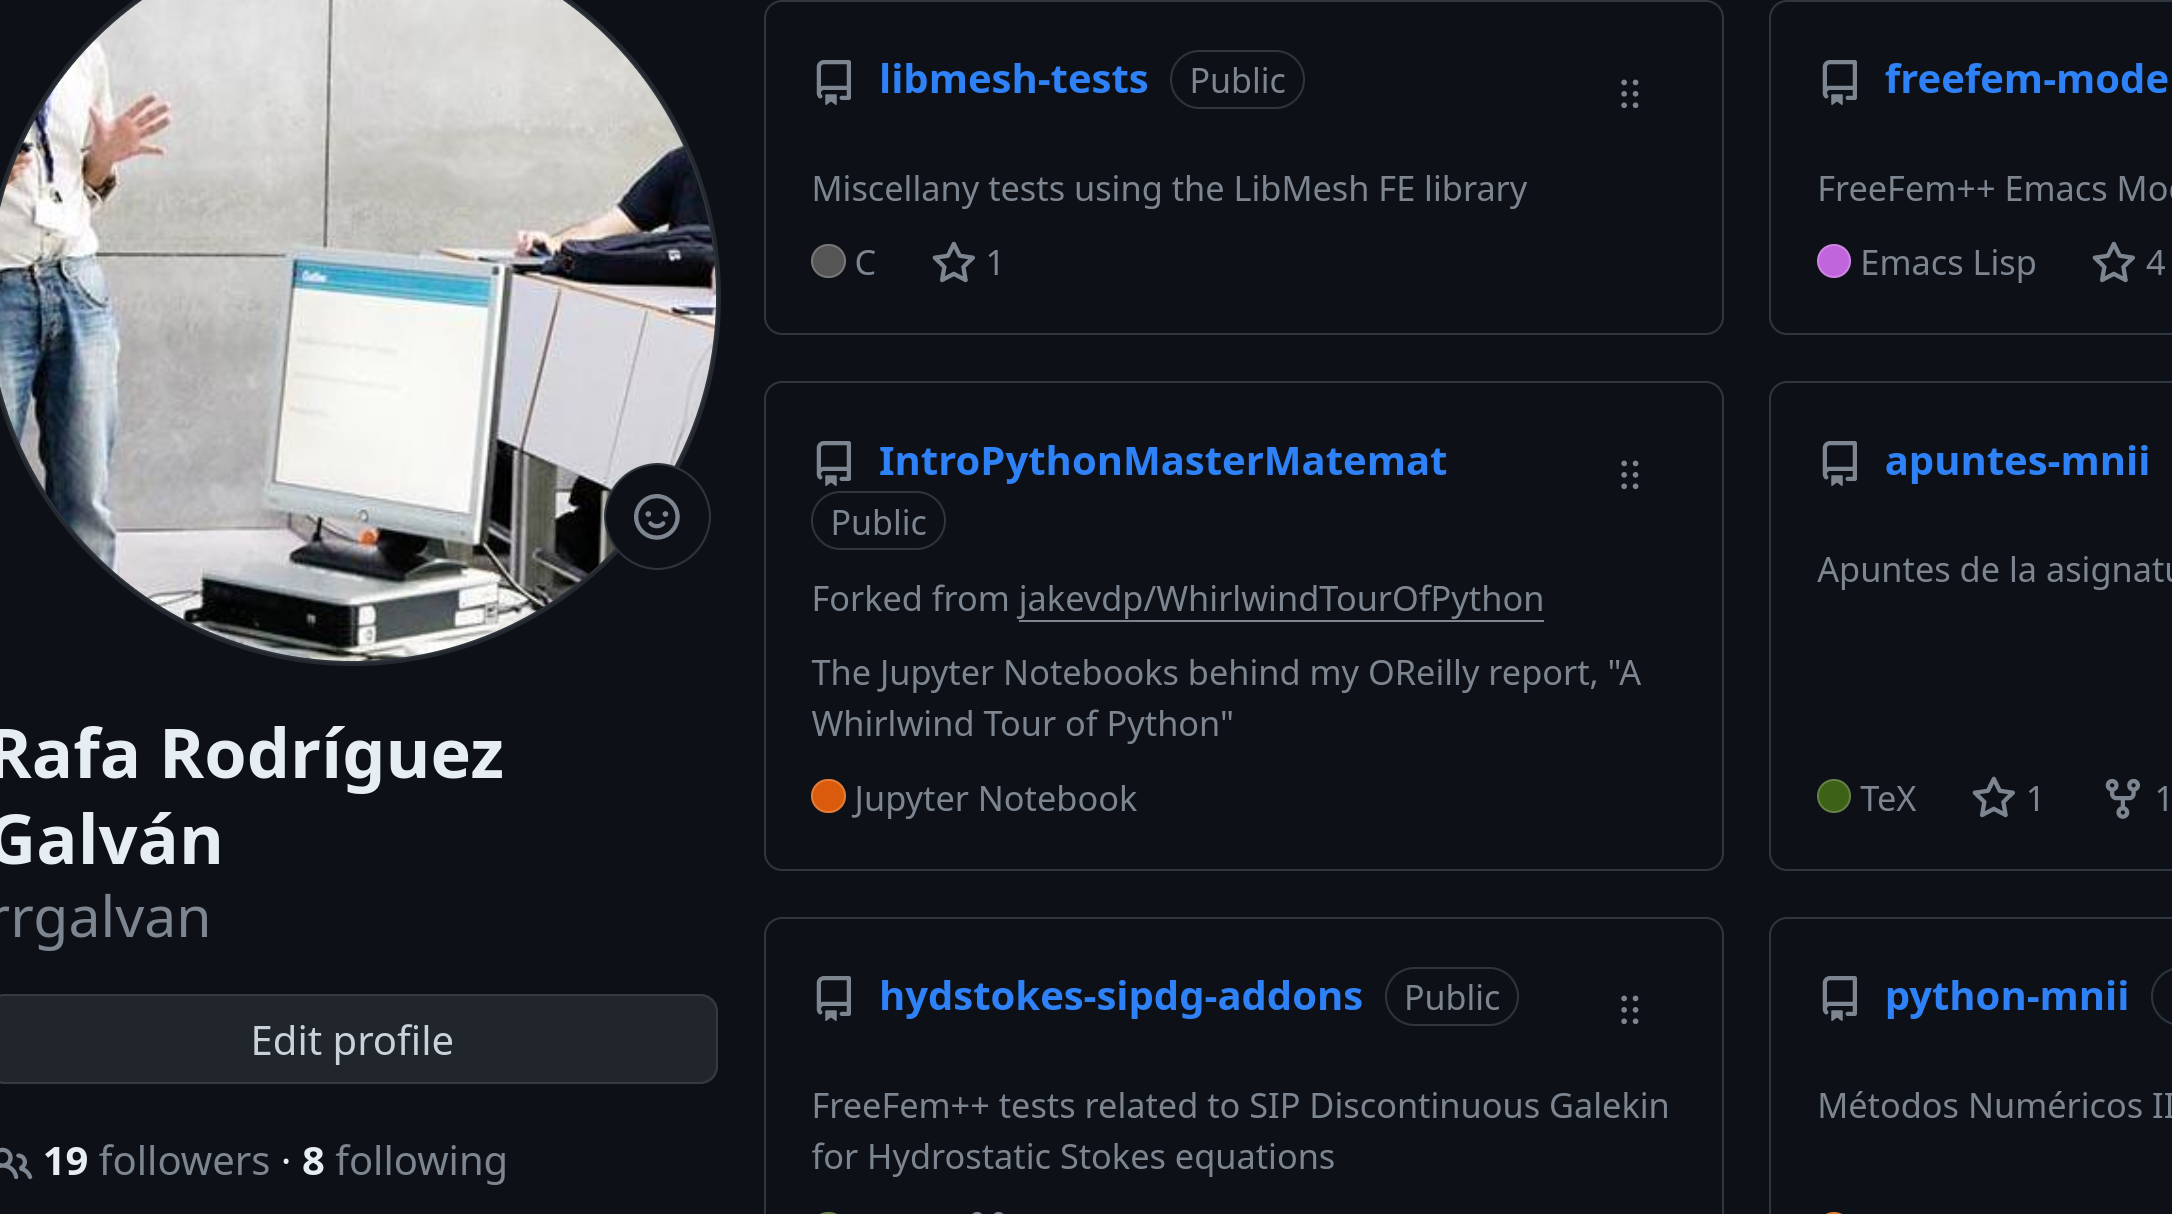
\includegraphics[width=0.40\linewidth]{img/github}
  \end{flushright}
\end{frame}

%===============================================================
\begin{frame}{Datos Abiertos (I)}
%---------------------------------------------------------------
  \vspace{-3.8em}
  \begin{itemize}
    \setlength\itemsep{0.4em}
    \item<1-> Muchos investigadores de la UCA \emph{usan grandes \par bases de datos} con licencia abierta
    \item<1-> También se \emph{generan bases de datos}, no siempre públicas o con licencia abierta \texttt{:-(}
  \begin{itemize}
    \item Modelo competitivo vs modelo colaborativo 
    \item ¿Las universidades incentivan la publicación de datos en abierto? 
  \end{itemize}
    \item<2-> ¿Cómo? Se suelen usar \emph{repositorios externos} como \structure{\url{https://figshare.com}}
    \item<3-> Reproducibilidad de los tests numéricos, publicación del código fuente en repositorios como Github. Tesis en abierto
  \end{itemize}
  \vspace{-7.0cm}
  \begin{flushright}
    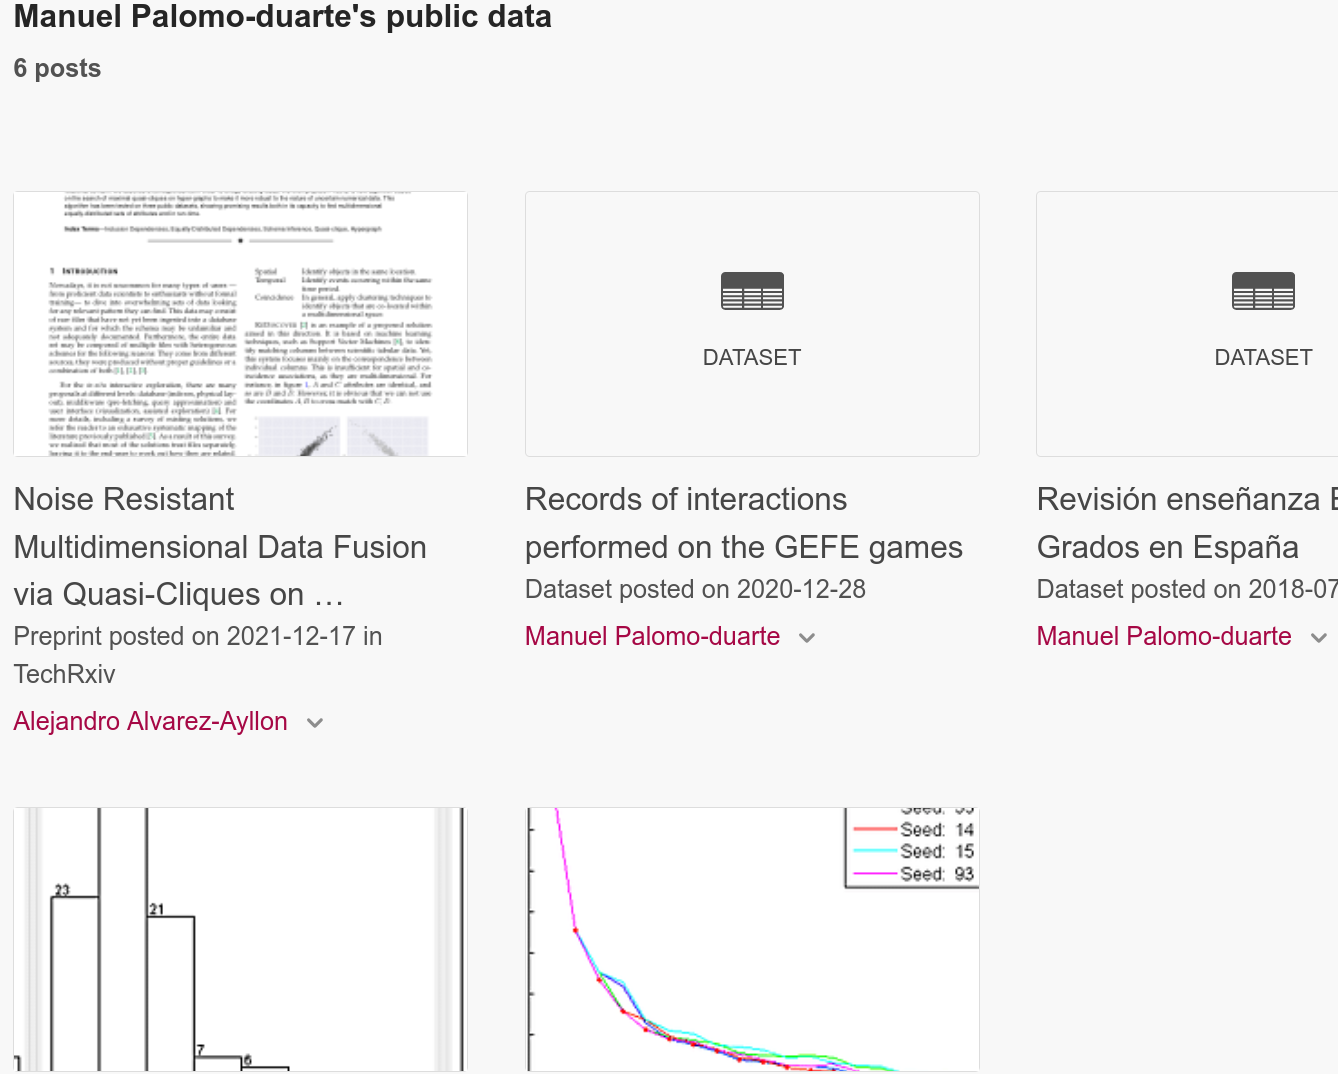
\includegraphics[width=0.26\linewidth]{img/figshare}
  \end{flushright}
\end{frame}

%===============================================================
\begin{frame}{Datos Abiertos (II). Inteligencia Artificial}
%---------------------------------------------------------------
  \vspace{-2.5cm}
  \begin{flushright}
    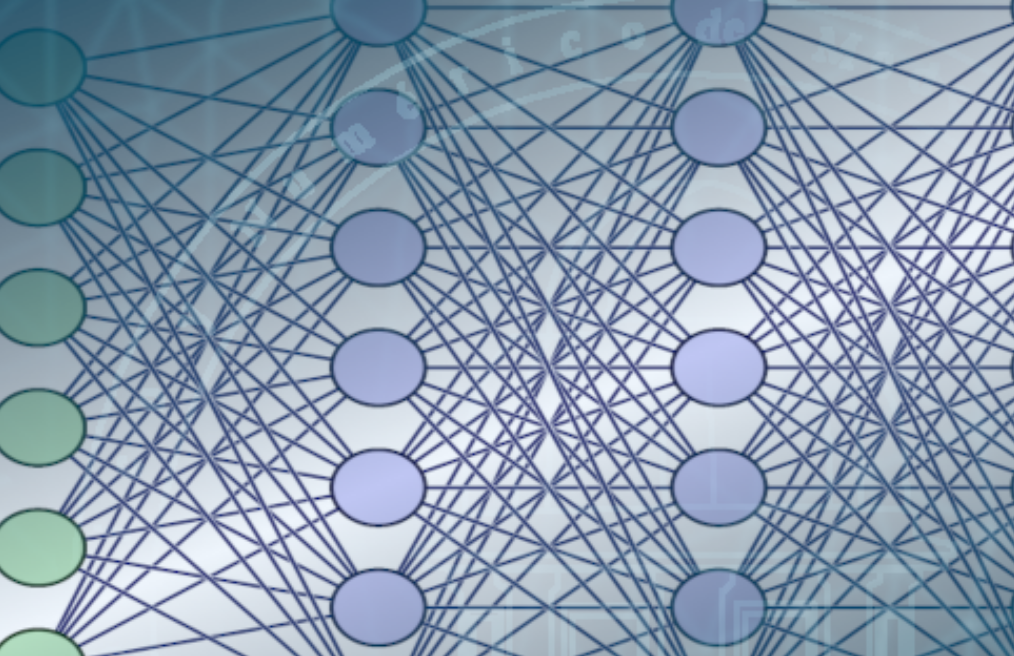
\includegraphics[width=0.26\linewidth]{img/NN}
  \end{flushright}
  \vspace{-1.0cm}
  Años recientes: interés por las \alert{redes neuronales} 
  \bigskip
  \begin{itemize}
    % \selength\itemsep{0.3em}
    \item Importancia de datos: entrenamiento, testado de la RN
    \item El poder de la combinación datos $+$ IA. OpenAI y ChatGPT, Google, Microsoft... 
    \item Pero siempre datos cerrados :-(
    \item Bibliotecas como \texttt{TensorFlow}, ofrecen bases de datos con licencia libre \url{https://github.com/tensorflow/datasets/}
    \item Necesidad de que las instituciones publicas abran los datos 
  \end{itemize}

\end{frame}


%===============================================================
\begin{frame}{Datos Abiertos (III). Datos Externos}
%---------------------------------------------------------------
  \vspace{-0.3cm}
  Ejemplo en la UCA: el proyecto \emph{\alert{Smart Shipping}}
  \bigskip
  \begin{itemize}
    \setlength\itemsep{0.3em}
    \item Orientado a la \structure{optimización de rutas marítimas}, usando \textbf{datos en tiempo real} (vientos, corrientes, etc) 
    \item Extraídos de \textbf{bases de datos} gratuitas y abiertas (\structure{Copernicus Marine Service}, Unión Europea), \url{https://marine.copernicus.eu}
    \item Los datos son vitales para el éxito del proyecto
  \end{itemize}

  \vspace{-8.0cm}
  \begin{flushright}
    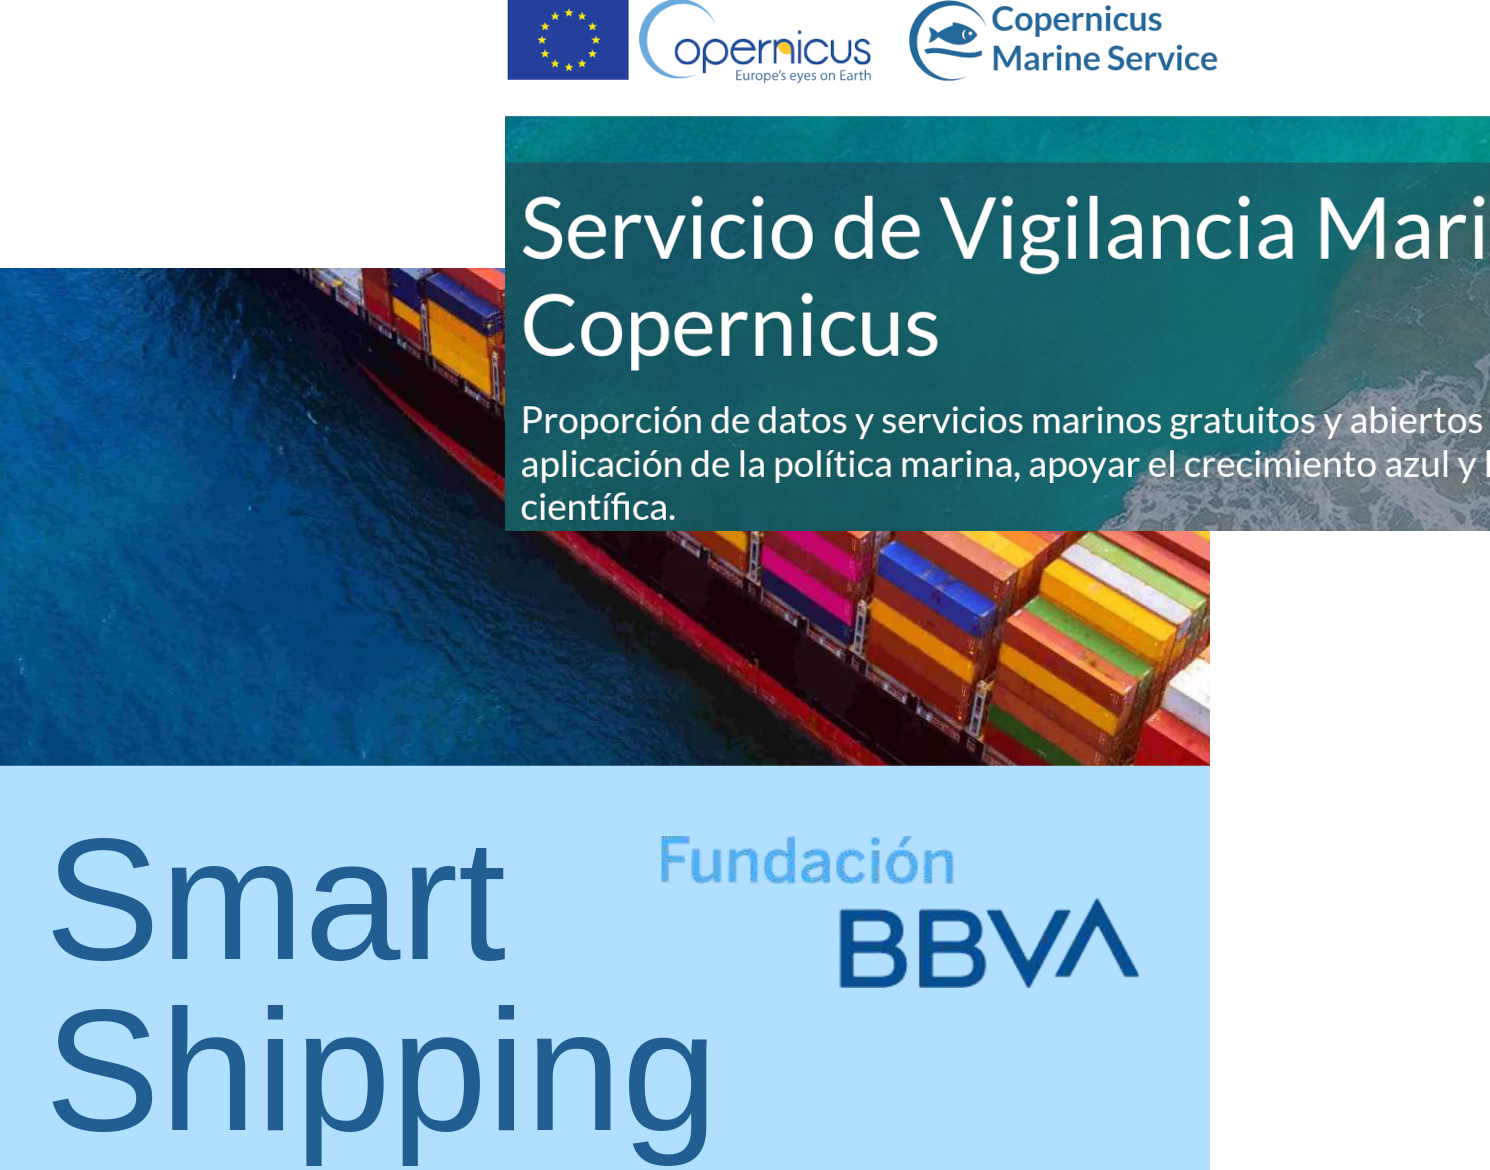
\includegraphics[width=0.40\linewidth]{img/smart-shipping}
  \end{flushright}
\end{frame}


%===============================================================
\begin{frame}{Publicaciones Científicas}
%---------------------------------------------------------------
  \vspace{-1.2cm}
  \begin{itemize}
    \setlength\itemsep{0.7em}
    \item<1-> La UCA promueve la \textit{publicación en abierto}
      \begin{itemize}
        \setlength\itemsep{0.2em}
        \item Supone multiplicar las posibilidades de difusión y el impacto 
        \item Biblioteca: \structure{Guía de publicación} en abierto
        \item \structure{Plan propio} estímulo y apoyo a Investigación: ayudas para publicación «Open Access» 
      \end{itemize}
    \item<2-> Publicación de \it{preprints}/\it{postprints}
      \begin{itemize}
        \setlength\itemsep{0.2em}
        \item \structure{RODIN} (biblioteca UCA), \structure{ArXiv} (repositorio para artículos científicos) 
        \item Ejemplo: «Mathematical Modelling of Neuroblast Chemotaxis Migration towards the Olfactory Bulb», \url{https://arxiv.org/abs/2211.06166}, \alert{licencia CC-BY-SA}.
  \end{itemize}
  \end{itemize}

  \vspace{-7.5cm}
  \begin{flushright}
    \fbox{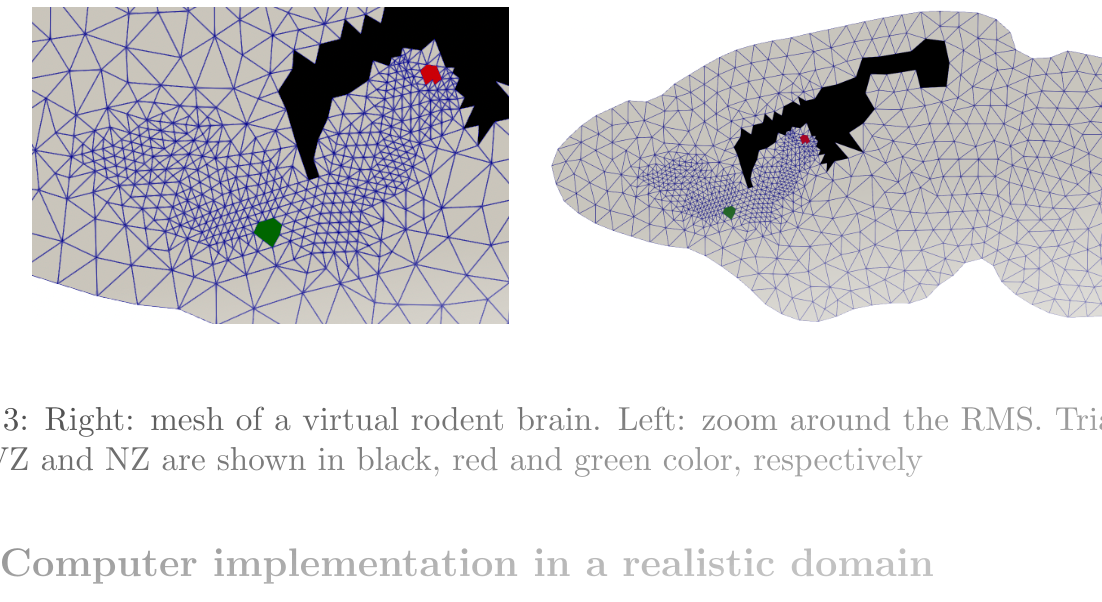
\includegraphics[width=0.38\linewidth]{img/neuroblastos}}
  \end{flushright}
\end{frame}


%===============================================================
\begin{frame}{}
%---------------------------------------------------------------
  \begin{center}
    \structure{\bf\Huge{¡Gracias!}}
  \end{center}
\end{frame}

\end{document}






%%% Local Variables:
%%% coding: utf-8
%%% TeX-master: t
%%% mode: latex
%%% ispell-local-dictionary: "english"
%%% End:
